\section{Surfaces}

\subsection{Basic definitions}
\begin{definition}
	A \vocab{topological surface} is a topological space $\Sigma$ such that
	\begin{enumerate}
		\item for all points $p \in \Sigma$, there exists an open neighbourhood $p \in U \subset \Sigma$ such that $U$ is homeomorphic to $\mathbb R^2$, or a disc $D^2 \subset \mathbb R^2$, with its usual Euclidean topology;
		\item $\Sigma$ is Hausdorff and second countable.
	\end{enumerate}
\end{definition}

\begin{definition}[Hausdorff]
	A space $X$ is \vocab{Hausdorff} if two points $p \neq q \in X$ have open neighbourhoods $U, V$ such that $U \cap V = \emptyset$.
\end{definition} 

\begin{definition}[Second Countable]
	A space $X$ is \vocab{second countable} if it has a countable base; there exists a countable family of open sets $U_i$, such that every open set is a union of some of the $U_i$.
\end{definition} 

\begin{remark} \
	\begin{enumerate}
		\item $\mathbb R^2$ is homeomorphic to the open disc $D(0,1) = \qty{ x \in \mathbb R^2 : \norm{x} < 1 }$.
		\item The first part of the definition is important whilst the second part (Hausdorff and second countable) is a technical point. 
		These topological requirements are typically not the purpose of considering topological spaces, but they are occasionally technical requirements to prove interesting theorems.
		\item 	Note that subspaces of Hausdorff and second countable spaces are also Hausdorff and second countable.	
		In particular, Euclidean space $\mathbb R^n$ is Hausdorff (as $\mathbb R^n$ is a metric space) and second countable (consider the set of balls $D(p,q)$ for points $p$ with rational coordinates, and rational radii $q$).
		Hence, any subspace of $\mathbb R^n$ is implicitly Hausdorff and second countable.
	\end{enumerate} 
\end{remark}

\begin{example}
	$\mathbb R^2$ is a topological surface.
	Any open subset of $\mathbb R^2$ is also a topological surface.
	For example, $\mathbb R^2 \setminus \qty{0}$ and $\mathbb R^2 \setminus \qty{(0,0)} \cup \qty{\qty(0, \frac{1}{n}) : n = 1, 2, \dots}$ are topological surfaces.
\end{example}

\begin{example}
	Let $f : \mathbb R^2 \to \mathbb R$ be a continuous function.
	The graph of $f$, denoted $\Gamma_f$, is defined by
	\begin{align*}
		\Gamma_f = \qty{(x,y,f(x,y)) : (x,y) \in \mathbb R^2} \subset \mathbb{R}^3
	\end{align*}
	with the subspace topology when embedded in $\mathbb R^3$.

	Recall that the product topology on $X \times Y$ for $X, Y$ topological spaces, has basic open sets $U \times V$, where $U \subset X$, $V \subset Y$ open.
	Also the product topology has the feature that $g : Z \to X \times Y$ is continuous iff $\pi_x \circ g : Z \to X$ and $\pi_y \circ f : Z \to Y$ are continuous\footnote{$\pi_x, \pi_y$ are the canonical projections, $\pi_x : X \times Y \to X$}.

	Hence, any graph $\Gamma \subseteq X \times Y$ is homeomorphic to $X$ if $f$ is continuous.
	Indeed, the projection $\pi_x$ projects each point in the graph onto the domain.
	The function $s : x \mapsto (x,f(x))$ is continuous as $\pi_x \circ s$ and $\pi_y \circ s$ are.
	So $\pi_x \mid_{\Gamma_f}$ and $s$ are inverse homeomorphisms.

	So, in our case, the graph $\Gamma_f$ is homeomorphic to $\mathbb R^2$, and so is a topological surface.
\end{example}

\begin{remark}
	As a topological surface, $\Gamma_f$ is independent of the function $f$.
	However, we will later introduce more ways to describe topological spaces that will ascribe new properties to $\Gamma_f$ which do depend on $f$.
\end{remark}

\begin{example}
	The sphere:
	\begin{align*}
		S^2 = \qty{(x,y,z) \in \mathbb R^3 : x^2 + y^2 + z^2 = 1}
	\end{align*}
	is a topological surface, when using the subspace topology in $\mathbb R^3$.

	This is a subspace of $\mathbb{R}^3$ so is Hausdorff and second countable.
	
	Consider the stereographic projection of $S^2$ onto $\mathbb R^2$ from the north pole $(0,0,1)$.
	The projection satisfies $\pi_+ : S^2 \setminus \qty{(0,0,1)}$ and
	\begin{align*}
		(x,y,z) \mapsto \qty(\frac{x}{1-z}, \frac{y}{1-z}).
	\end{align*}
	Certainly, $\pi_+$ is continuous, since we do not consider the point $(0,0,1)$ to be in its domain.
	The inverse map is given by
	\begin{align*}
		(u,v) \mapsto \qty(\frac{2u}{u^2+v^2+1}, \frac{2v}{u^2+v^2+1}, \frac{u^2+v^2-1}{u^2+v^2+1}).
	\end{align*}
	This is also a continuous function.
	Hence $\pi_+$ is a homeomorphism.

	Similarly, we can construct the stereographic projection from the south pole, $\pi_-: S^2 \setminus \qty{(0,0,-1)} \to \mathbb{R}^2$.
	\begin{align*}
		(x,y,z) \mapsto \qty(\frac{x}{1+z}, \frac{y}{1+z}).
	\end{align*}
	This is a homeomorphism.

	Hence, every point in $S^2$ lies either in the domain of $\pi_+$ or $\pi_-$, and hence sits in an open set $S^2 \setminus \qty{(0,0,1)}$ or $S^2 \setminus \qty{(0,0,-1)}$ which are homeomorphic to $\mathbb R^2$.
	So $S^2$ is a topological surface.
\end{example}

\begin{remark}
	$S^2$ is compact by the Heine-Borel theorem; it is a closed bounded set in $\mathbb R^3$.
\end{remark}

\begin{example}
	The real projective plane is a topological surface.

	The group $\mathbb Z_2$ acts on $S^2$ by homeomorphisms via the \textit{antipodal map} $a : S^2 \to S^2$, mapping $x \mapsto -x$.
	So $\mathbb{Z}_2$ sits in the group of homeomorphisms of $S^2$, $\mathrm{Homeo}(S^2)$, as we can map $-1 \to a$.

	\begin{definition}[The Real Projective Plane]
		The real projective plane, $\mathbb{R} \mathbb{P}^2$, is the quotient of $S^2$ given by identifying every point $x$ with its image $-x$ under $a$.
		\begin{align*}
			\mathbb R \mathbb P^2 = \faktor{S^2}{\mathbb Z_2} = \faktor{S^2}{\sim};\quad x \sim a(x)
		\end{align*}
	\end{definition} 

	\begin{lemma}
		As a set, $\mathbb R \mathbb P^2$ naturally bijects with the set of straight lines in $\mathbb R^3$ through the origin.
	\end{lemma}

	\begin{proof}
		Any line through the origin intersects $S^2$ exactly in a pair of antipodal points $x, -x$.
		Similarly, pairs of antipodal points uniquely define a line through the origin.
	\end{proof}
	
	\begin{lemma}
		$\mathbb R \mathbb P^2$ is a topological surface with the \underline{quotient topology}.
	\end{lemma}

	Recall: Quotient topology : $q : X \to Y$ ($q$ the quotient map), $V \subset Y$ is open iff $q\inv V \subset X$ is open in $X$(i.e. iff $q$ is continuous).
	
	\begin{proof}
		We must check that $\mathbb R \mathbb P^2$ is Hausdorff since it is constructed by a quotient, not a subspace. \\
		If $[p] \neq [m] \in \mathbb R \mathbb P^2$, then $\pm p, \pm m \in S^2$ are distinct antipodal pairs.
		We can therefore construct distinct open discs\footnote{Just take a ball in $\mathbb{R}^3$ and intersect with $S^2$} around $p, m$ in $S^2$, and their antipodal images.
		These uniquely define open neighbourhoods of $[p], [q]$, which are disjoint, as for $q : S^2 \to \mathbb{R} \mathbb{P}^2$, $q(B_\delta(p))$ is \underline{open} since $q\inv(q(B_\delta(p))) = B_\delta(p) \cup (-B_\delta(p))$ is open.

		Similarly, we can check that $\mathbb R \mathbb P^2$ is second countable. \\
		We know that $S^2$ is second countable, so let $\mathcal U_0$ be a countable base for the topology on $S^2$.
		Let $\overline{\mathcal U_0} = \{q(u) : u \in \mathcal{U}_0\}$.
		$q(u)$ is open as $q\inv(q(u)) = u \cup (-u)$ is open. 
		$\overline{\mathcal U_0}$ is clearly countable since $\mathcal{U}_0$ is.
		Now, if $V \subset \mathbb R \mathbb P^2$ is open, then by definition of quotient topology $q^{-1}(V)$ is open in $S^2$ hence $q^{-1}(V) = \cup_\alpha U_\alpha, U_\alpha \in \mathcal{U}_0$.
		$V = q(q\inv V) = q(\cup_\alpha U_\alpha) = \cup_\alpha q(U_\alpha), q(U_\alpha) \in \overline{\mathcal{U}_0}$.

		Finally, let $p \in S^2$ and $[p] \in \mathbb R \mathbb P^2$ its image.
		Let $\overline D$ be a small (contained in an open hemisphere) closed disc, which is a neighbourhood of $p \in S^2$.
		The quotient map restricted to $\overline D$, written $\eval{q}_{\overline D} : \overline D \to q(\overline D) \subset \mathbb R \mathbb P^2$, is a continuous function from a \underline{compact} space to a \underline{Hausdorff} space.
		Further, $q$ is \underline{injective} on $\overline D$ since the disc was contained entirely in a single hemisphere so it cannot contain antipodal points. \\
		Recall from AT that the ``topological inverse function theorem" (TIFT) states that a continuous bijection from a compact space to a Hausdorff space is a \underline{homeomorphism}.\footnote{A brief proof is we want to show the inverse function is continuous, so it maps closed sets to closed sets. Take a closed set inside compact space so its compact, apply the continuous function to it so the image is compact. A compact set in a Hausdorff space is closed.} \\
		So $\eval{q}_{\overline D}$ is a homeomorphism from $\overline D$ to $q(\overline D)$.
		This then induces the homeomorphism $\eval{q}_{D} : D \to q(D)$ where $D$ is an open disc, the interior of $\overline D$.
		So by construction, $[p] \in q(D)$ has an open neighbourhood in $\mathbb R \mathbb P^2$ which is homeomorphic to an open disc on $S^2$ and so to $\mathbb{R}^2$, concluding the proof.
	\end{proof}
\end{example}
\begin{example}
	Let $S^1 = \{z \in \mathbb{C} : |z| = 1\}$ be the unit circle in $\mathbb C$, and then we define the torus to be the product space $S^1 \times S^1$, with the subspace topology from $\mathbb C^2$ (which is identical to the product topology).
	\begin{lemma}
		The torus is a topological surface.
	\end{lemma}
	\begin{proof}
		Consider the map $e : \mathbb R^2 \to S^1 \times S^1 \subset \mathbb{C} \times \mathbb{C}$ defined by
		\begin{align*}
			(s,t) \mapsto \qty(e^{2\pi i s}, e^{2 \pi i t})
		\end{align*}
		We have an equivalence relation on $\mathbb{R}^2$ given by translations by $\mathbb{Z}^2$ as $e$ is constant under them.
		This induces a map $\hat e$ from $\faktor{\mathbb R^2}{\mathbb Z^2}$.

		% https://tikzcd.yichuanshen.de/#N4Igdg9gJgpgziAXAbVABwnAlgFyxMJZABgBpiBdUkANwEMAbAVxiRAB12BbOnACwBGAgAQAlAHoAmEAF9S6TLnyEUARnJVajFmwDK41cM54u8YftWz5IDNjwEiZVZvrNWiDuwBmAJzoBjYE4efiExKRkg7l5BEQAtCNlNGCgAc3giUF8ILiQyEBwIJElqVx0PAEcQagY6ARgGAAVFexUQHyxUvhwrLJ8cvOpCpHUtNzZWOT6BxBKCosRRsvdPPl5hSYoZIA
		% Don't render this if we're hiding proofs anyway.
		\begin{center}
			\ifdefined\hideproofs
			\else
			\begin{tikzcd}
				\mathbb R^2 \arrow[d, "q"'] \arrow[r, "e"]             & S^1 \times S^1 \\
				\faktor{\mathbb R^2}{\mathbb Z^2} \arrow[ru, "\hat e"] &
			\end{tikzcd}
			\fi
		\end{center}

		Under the quotient topology given by the quotient map $q$, $\faktor{\mathbb R^2}{\mathbb Z^2}$ is a topological space.
		The map $[0,1]^2 \to \mathbb R^2 \to \faktor{\mathbb R^2}{\mathbb Z^2}$ is surjective, so $\faktor{\mathbb R^2}{\mathbb Z^2}$ is compact.
		As $e$ is constant on an equivalence class, $\hat e$ is a continuous map from a compact space to a Hausdorff space, and $\hat e$ is bijective, so $\hat e$ is a homeomorphism by TIFT.

		We already have that $S^1 \times S^1$ is compact and Hausdorff (as a closed and bounded set in $\mathbb C^2$, equivalent to $\mathbb{R}^4$), so it suffices to show it is locally homeomorphic to $\mathbb R^2$.

		Similarly to the case of $S^2 \to \mathbb{R} \mathbb{P}^2$, pick $[p] \in q(p), p \in \mathbb{R}^2$, then we can choose a small closed disc $\overline D(p) \subset \mathbb{R}^2$ such that $\overline D(p) \cap \qty(\overline D(p) + (n,m)) = \varnothing$ for all nonzero $(n,m) \in \mathbb Z^2$.
		Hence $\eval{e}_{\overline D(p)}$ and $\eval{q}_{\overline D(p)}$ are injective.
		Now, restricting to the open disc as before, we can find an open disc neighbourhood of $[p] \in \faktor{\mathbb R^2}{\mathbb Z^2}$.
		Since $[p]$ was chosen arbitrarily, $S^1 \times S^1$ is a topological surface.
	\end{proof}

	Another viewpoint: \\
	$\faktor{\mathbb R^2}{\mathbb Z^2}$ is also given by imposing on $[0, 1]^2$ the equivalence  relation
	\begin{align*}
		(x, 0) &\sim (x, 1) \quad \forall \; 0 \leq x \leq 1\\
		(0, y) &\sim (1, y) \quad \forall \; 0 \leq y \leq 1.
	\end{align*} 
\end{example}

\begin{example}
	Let $P$ be a planar Euclidean polygon (including interior), with oriented edges.
	We will pair the edges, and without loss of generality we will assume that paired edges have the same Euclidean length.
	\begin{center}
		\tikzfig{torus_polygon}
		\quad
		\tikzfig{other_square_polygon}
		\quad
		\tikzfig{hexagon}
	\end{center}
	We can assign letter names to each edge pair, and denote a polygon by the sequence of edges found when traversing in a clockwise orientation.
	The edge pair name is inverted if the edge is traversed in the reverse direction.
	Note the difference between the annotations on the first two shapes above, due to the reversed direction of the edge.

	If two edges $\{e, \hat e\}$ are paired, this defines a unique Euclidean isometry from $e$ to $\hat e$ respecting the orientation, which will be written $f_{e\hat e} : e \to \hat e$. \\
	The set of all such functions generate an equivalence relation on the polygon $P$, where we identify $x \in \partial P$ (a point on the boundary) with $f_{e \hat{e}}(x)$ whenever $x \in e$.

	\begin{lemma}
		$\faktor{P}{\sim}$, with the quotient topology, is a topological surface.
	\end{lemma}
\end{example}

\begin{example}
	Consider the torus, defined here as $T^2 = \faktor{[0,1]^2}{\sim}$.
	\begin{center}
		\tikzfig{torus_polygon}
	\end{center}
	Let $P$ be the polygon $[0,1]^2$.

	If $p$ is in the interior of $P$, then we pick $\delta > 0$ small s.t. $\overline{B_{\delta}(p)}$\footnote{The closure of $B_\delta(p)$} lies in the interior of $P$.
	Arguing as before in $\mathbb{R} \mathbb{P}^2$, the quotient map is injective on $\overline{B_{\delta}(p)}$ and is a homeomorphism on its interior.
	{ 	\par
		\centering 
		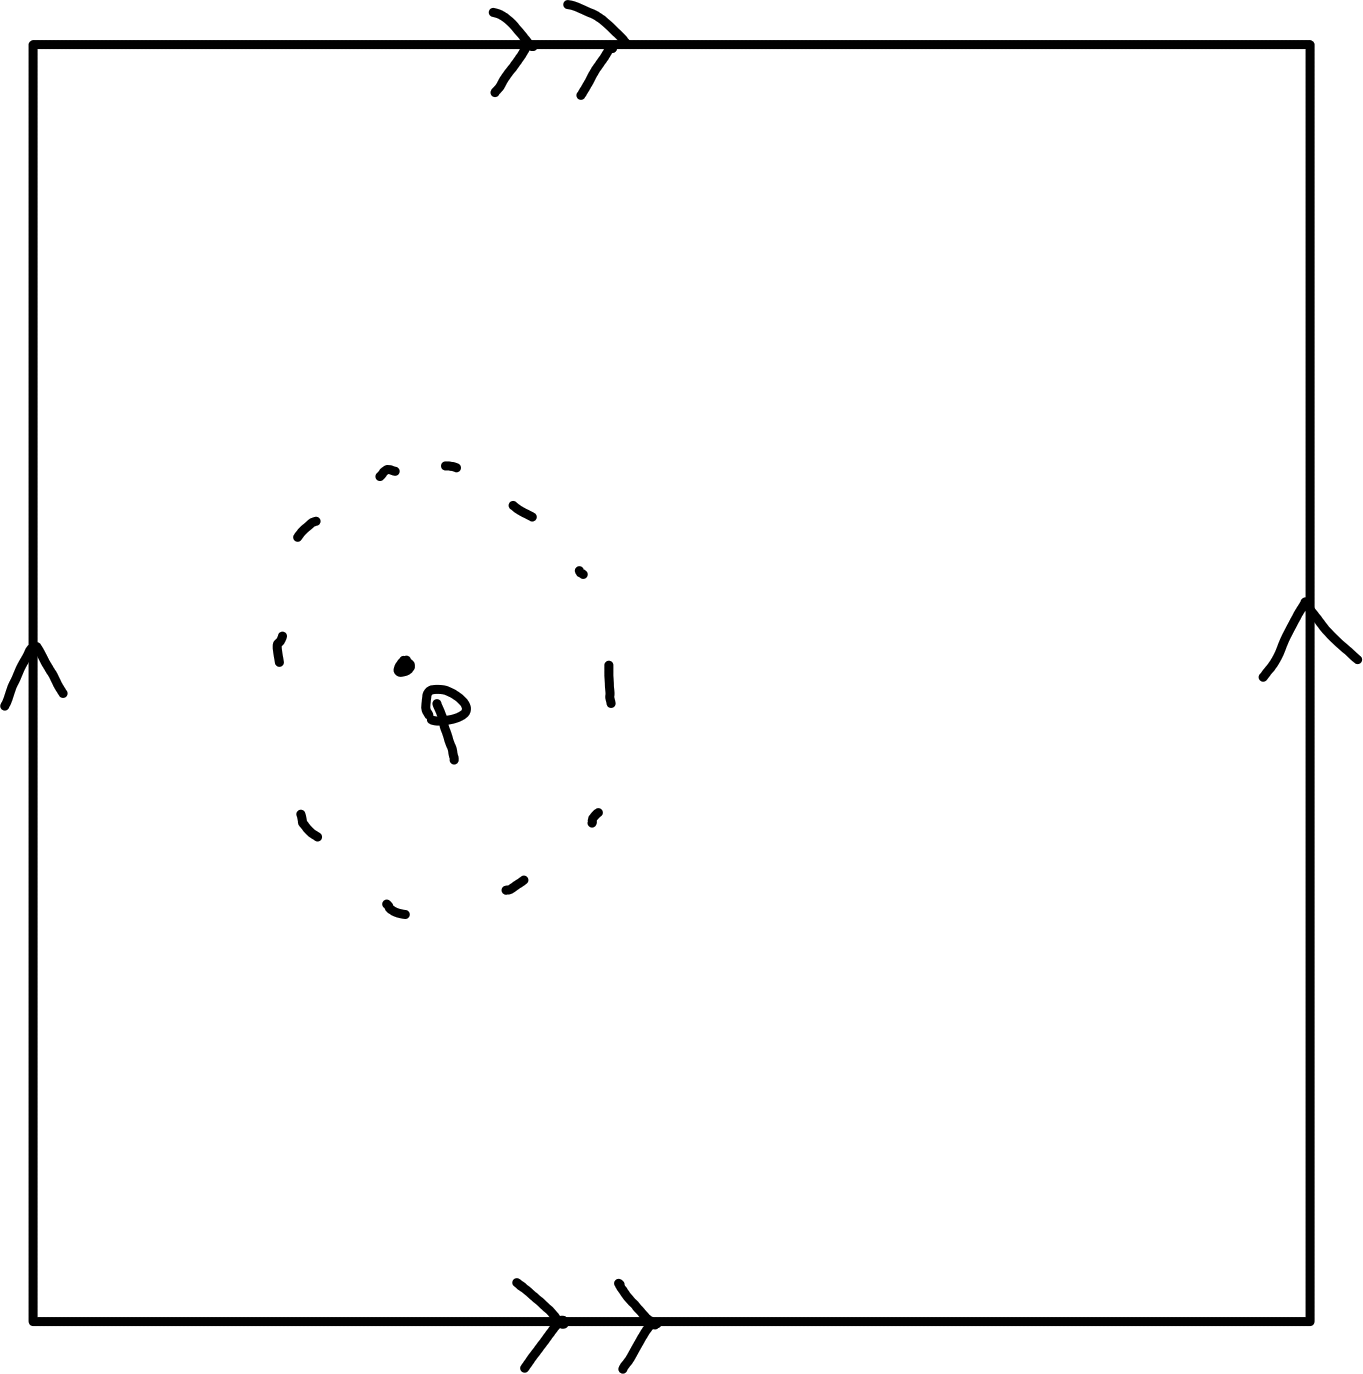
\includegraphics[height=3.5cm]{01-torussquare} 
		\par
	}

	Let $p$ be on an edge, but not a vertex.
	{ 	\par
		\centering 
		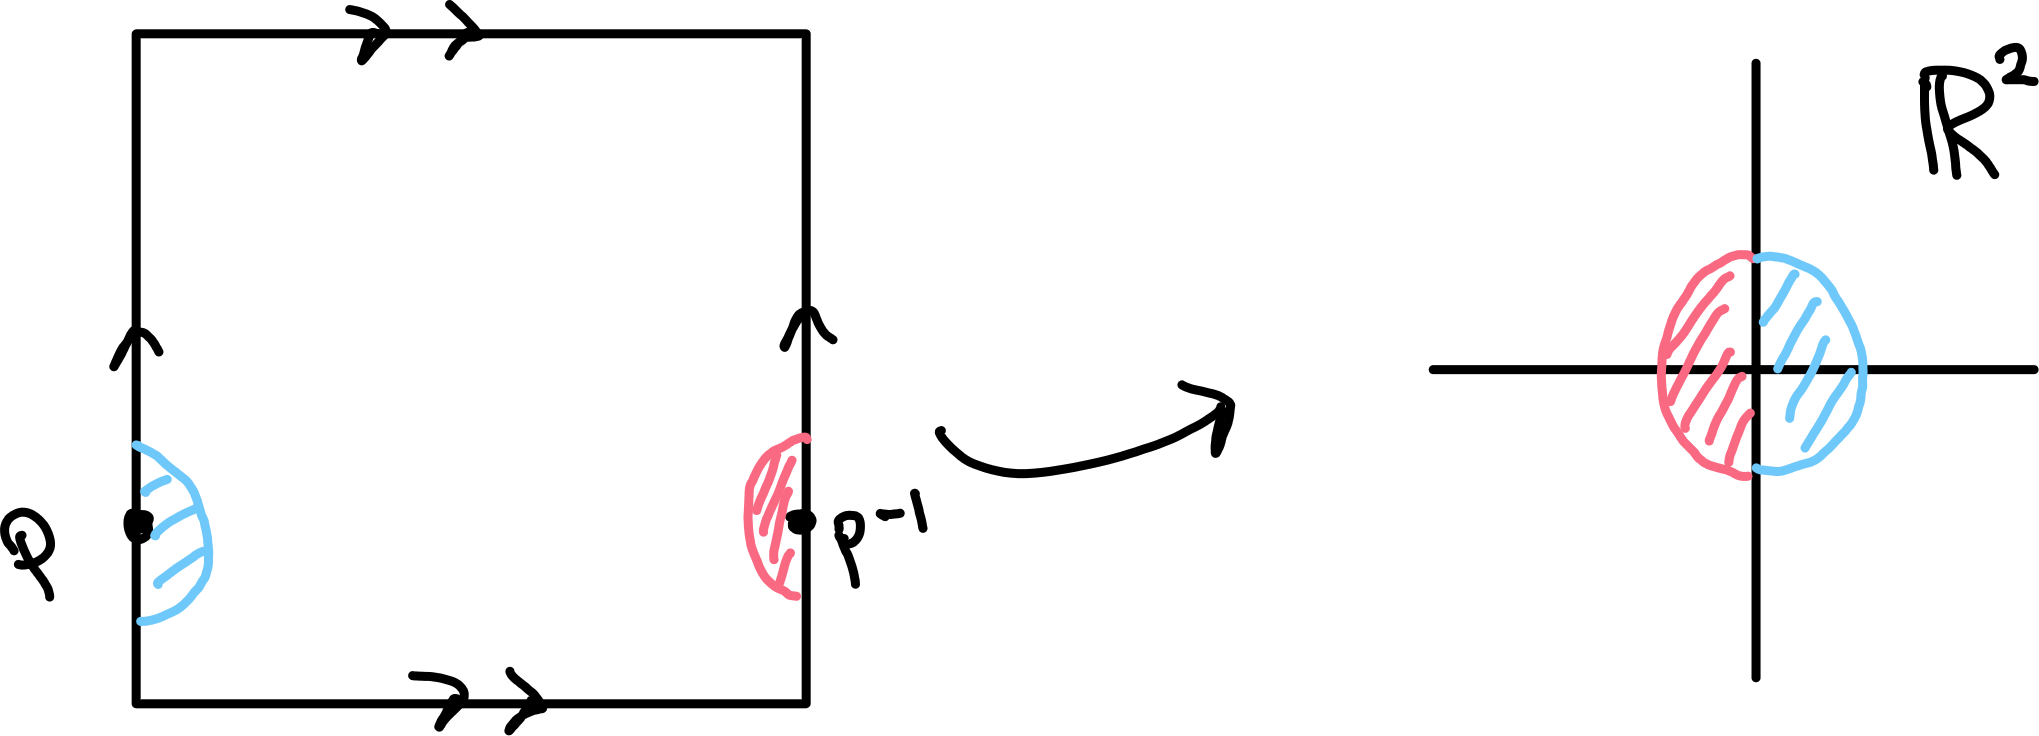
\includegraphics[height=5cm]{01-torussquare2} 
		\par
	}
	Let us say without loss of generality that $p = (0,y_0) \sim (1,y_0) = p'$.
	Let $\delta$ be sufficiently small that the closed half-discs $U, V$ centred on $p, p\inv$ with radius $\delta$ do not intersect any vertices. \\
	Then we define a map from the union of the two half-discs to the disc $B(0,\delta) \subseteq \mathbb R^2$ via 
	\begin{align*}
		U : (x,y) &\underset{f_u}{\mapsto} (x,y-y_0) \\
		V : (x,y) &\underset{f_v}{\mapsto} (x-1,y-y_0)
	\end{align*} which will be a bijective map.

	Recall the gluing lemma from Analysis and Topology: that if $X = A \cup B$ is a union of closed subspaces, and $f : A \to Y$, $g : B \to Y$ are continuous and $\eval{f}_{A \cap B} = \eval{g}_{A \cap B}$, they define a continuous map on $X$.

	$f_U, f_V$ are continuous on $U, V \subset [0, 1]^2$.
	By the definition of the quotient topology, $q \circ f_U$ and $q \circ f_V$ are also continuous ($q: [0, 1]^2 \to \faktor{[0, 1]^2}{\sim}$). \\
	In $T^2$, 1/2-discs, $q \circ U, q \circ V$ overlap but our maps agree as they are compatible with the equivalence relation. \\
	Hence, by the gluing lemma, $f_U, f_V$ ``glue'' together to give a continuous map to an open neighbourhood of $[p] \in T^2$ to $\mathbb{R}^2$.

	We can show that this is a homeomorphism using the usual process: pass to a closed disc, apply the topological inverse function theorem, then apply the result to the interior.
	If $[p] \in T^2$ lies in an edge on $P$, it has a neighbourhood homeomorphic to a disc.

	Now it suffices to consider points $p$ on a vertex.
	All four vertices of the square are identified to the same point in the torus as each vertex lies on two edges and so is identified to two other vertices.
	{ 	
		\par
		\centering 
		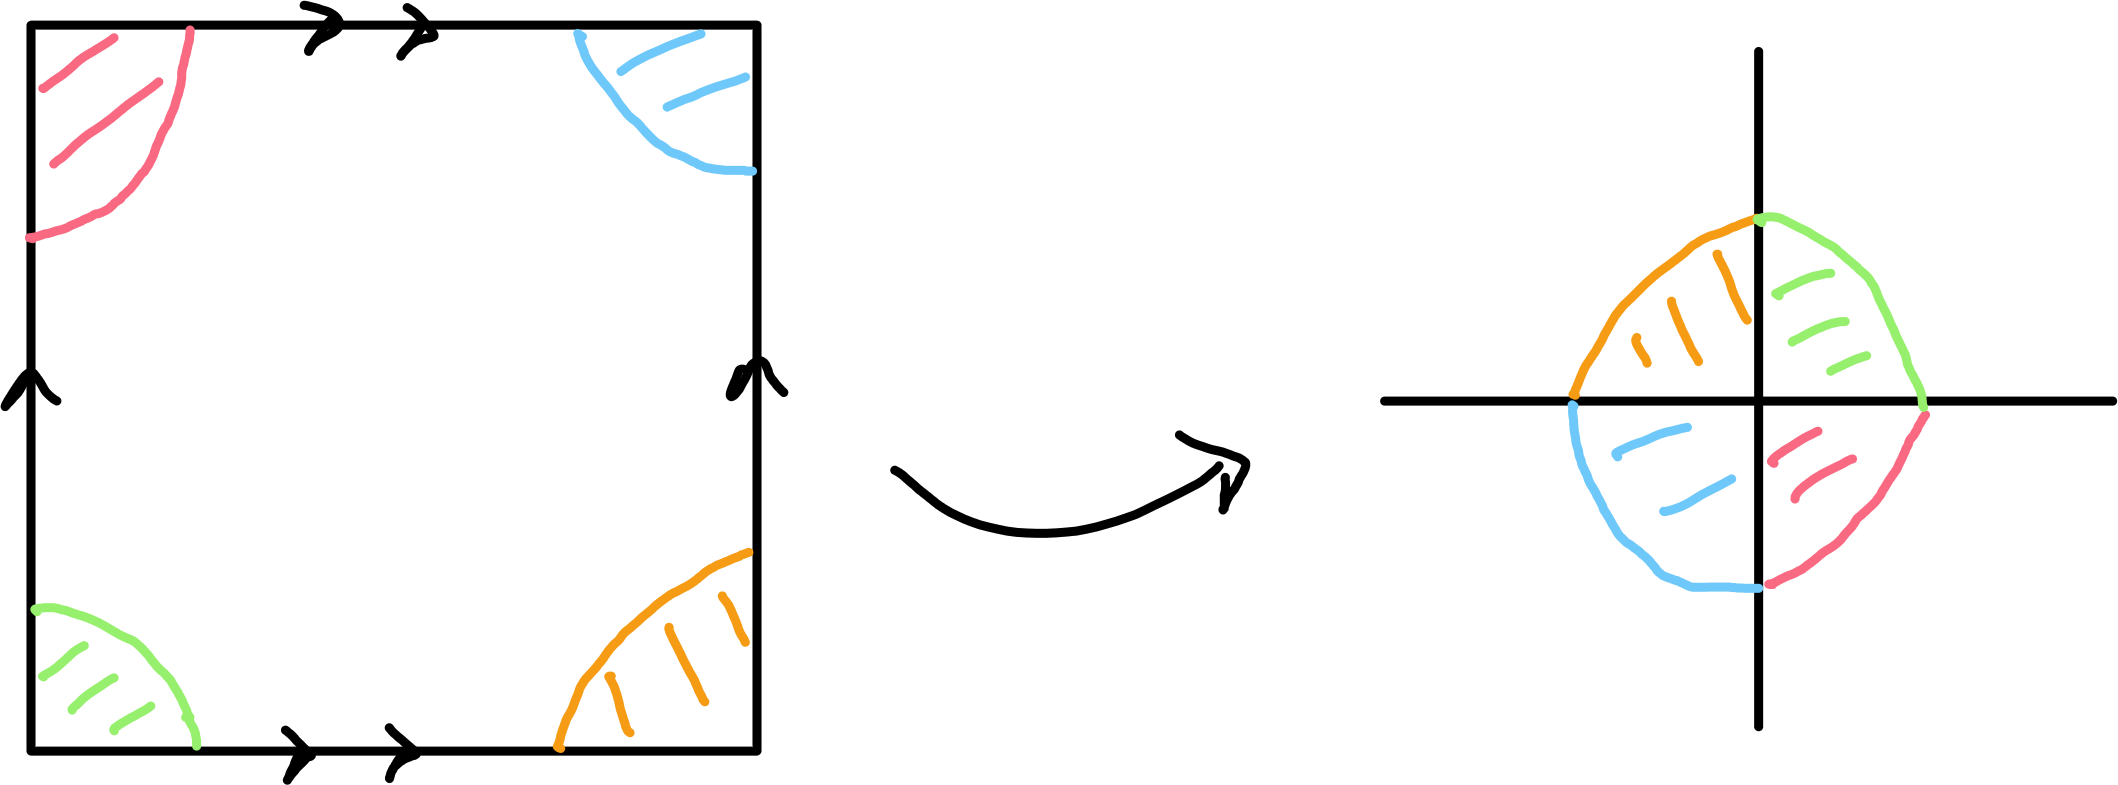
\includegraphics[height=5cm]{01-torussquare3} 
		\par
	}
	and analogously we get that a vertex has a neighbourhood homeomorphic to a disc.
	% A neighbourhood of each vertex can be identified with a quarter-disc in $\mathbb R^2$.
	% We can repeatedly apply the gluing lemma to construct the whole disc $B(0,\delta) \subseteq \mathbb R^2$ and complete the argument as before.

	Thus, $\faktor{[0,1]^2}{\sim}$ is a topological surface.
\end{example}

\begin{example}[General Polygon]
	We can generalise this proof to an arbitrary planar Euclidean polygon $P$, such as the hexagon above.
	The equivalence relation $x \sim f_{e \hat e}(x)$ induces an equivalence relation on the vertices of $P$, by considering the images of the vertices under all $f_{e\hat e}$.
	However, it is not necessarily the case that an equivalence class of vertices contains exactly four vertices, so quarter-discs are not necessarily applicable.
	Again, there are three types of point:
	\begin{itemize}
		\item interior points, for which a neighbourhood not intersecting the boundary is chosen;
		\item points on edges, for which a corresponding point exists and two half-discs can be glued to form the neighbourhood; and
		\item points on vertices.
		      For this case, all vertices of the polygon have a neighbourhood which is a sector of a circle.
		      Let there be $r$ vertices in a given equivalence class.
		      Let $\alpha$ be the sum of the angles of the sectors in a given class. \\
		      Any sector can be identified with a given sector in the disc $B(0,\delta) \subseteq \mathbb R^2$, which we will choose to have angle $\alpha / r$.
		      Then, we can glue each sector together in $\mathbb R^2$, compatibly with the orientations of the edges and arrows, inducing a neighbourhood which is locally homeomorphic to a disc.

		      If $r = 1$, we have an equivalence class comprising a single vertex, which gives a single sector.
		      For $r$ to be one, the two edges attached to this vertex must be paired and have the same direction (either both inwards or outwards from the vertex).
		      This quotient space is simply a cone, which is homeomorphic to a disc as required.
	\end{itemize}
	We can also show that the quotient space is Hausdorff and second countable.
	By construction, two distinct points in the quotient space can be separated by open neighbourhoods by selecting a sufficiently small radius such that the discs considered in the derivation above are disjoint.
	For second countability, consider
	\begin{itemize}
		\item discs in the interior of $P$ with rational centres and radii;
		\item for each edge of $P$, consider an isometry $e \to [0, \ell]$ where $\ell$ is the length of $e$, taking discs on $e$ which are centred at rational values in $[0,\ell]$; and
		\item for each vertex, consider discs centred at these vertices with rational radii.
	\end{itemize}
\end{example}

\begin{example}[Connected Sums]
	Given topological surfaces $\Sigma_1, \Sigma_2$ we can remove an open disc from each and glue the resulting boundary circles.
	{ 	
		\par
		\centering 
		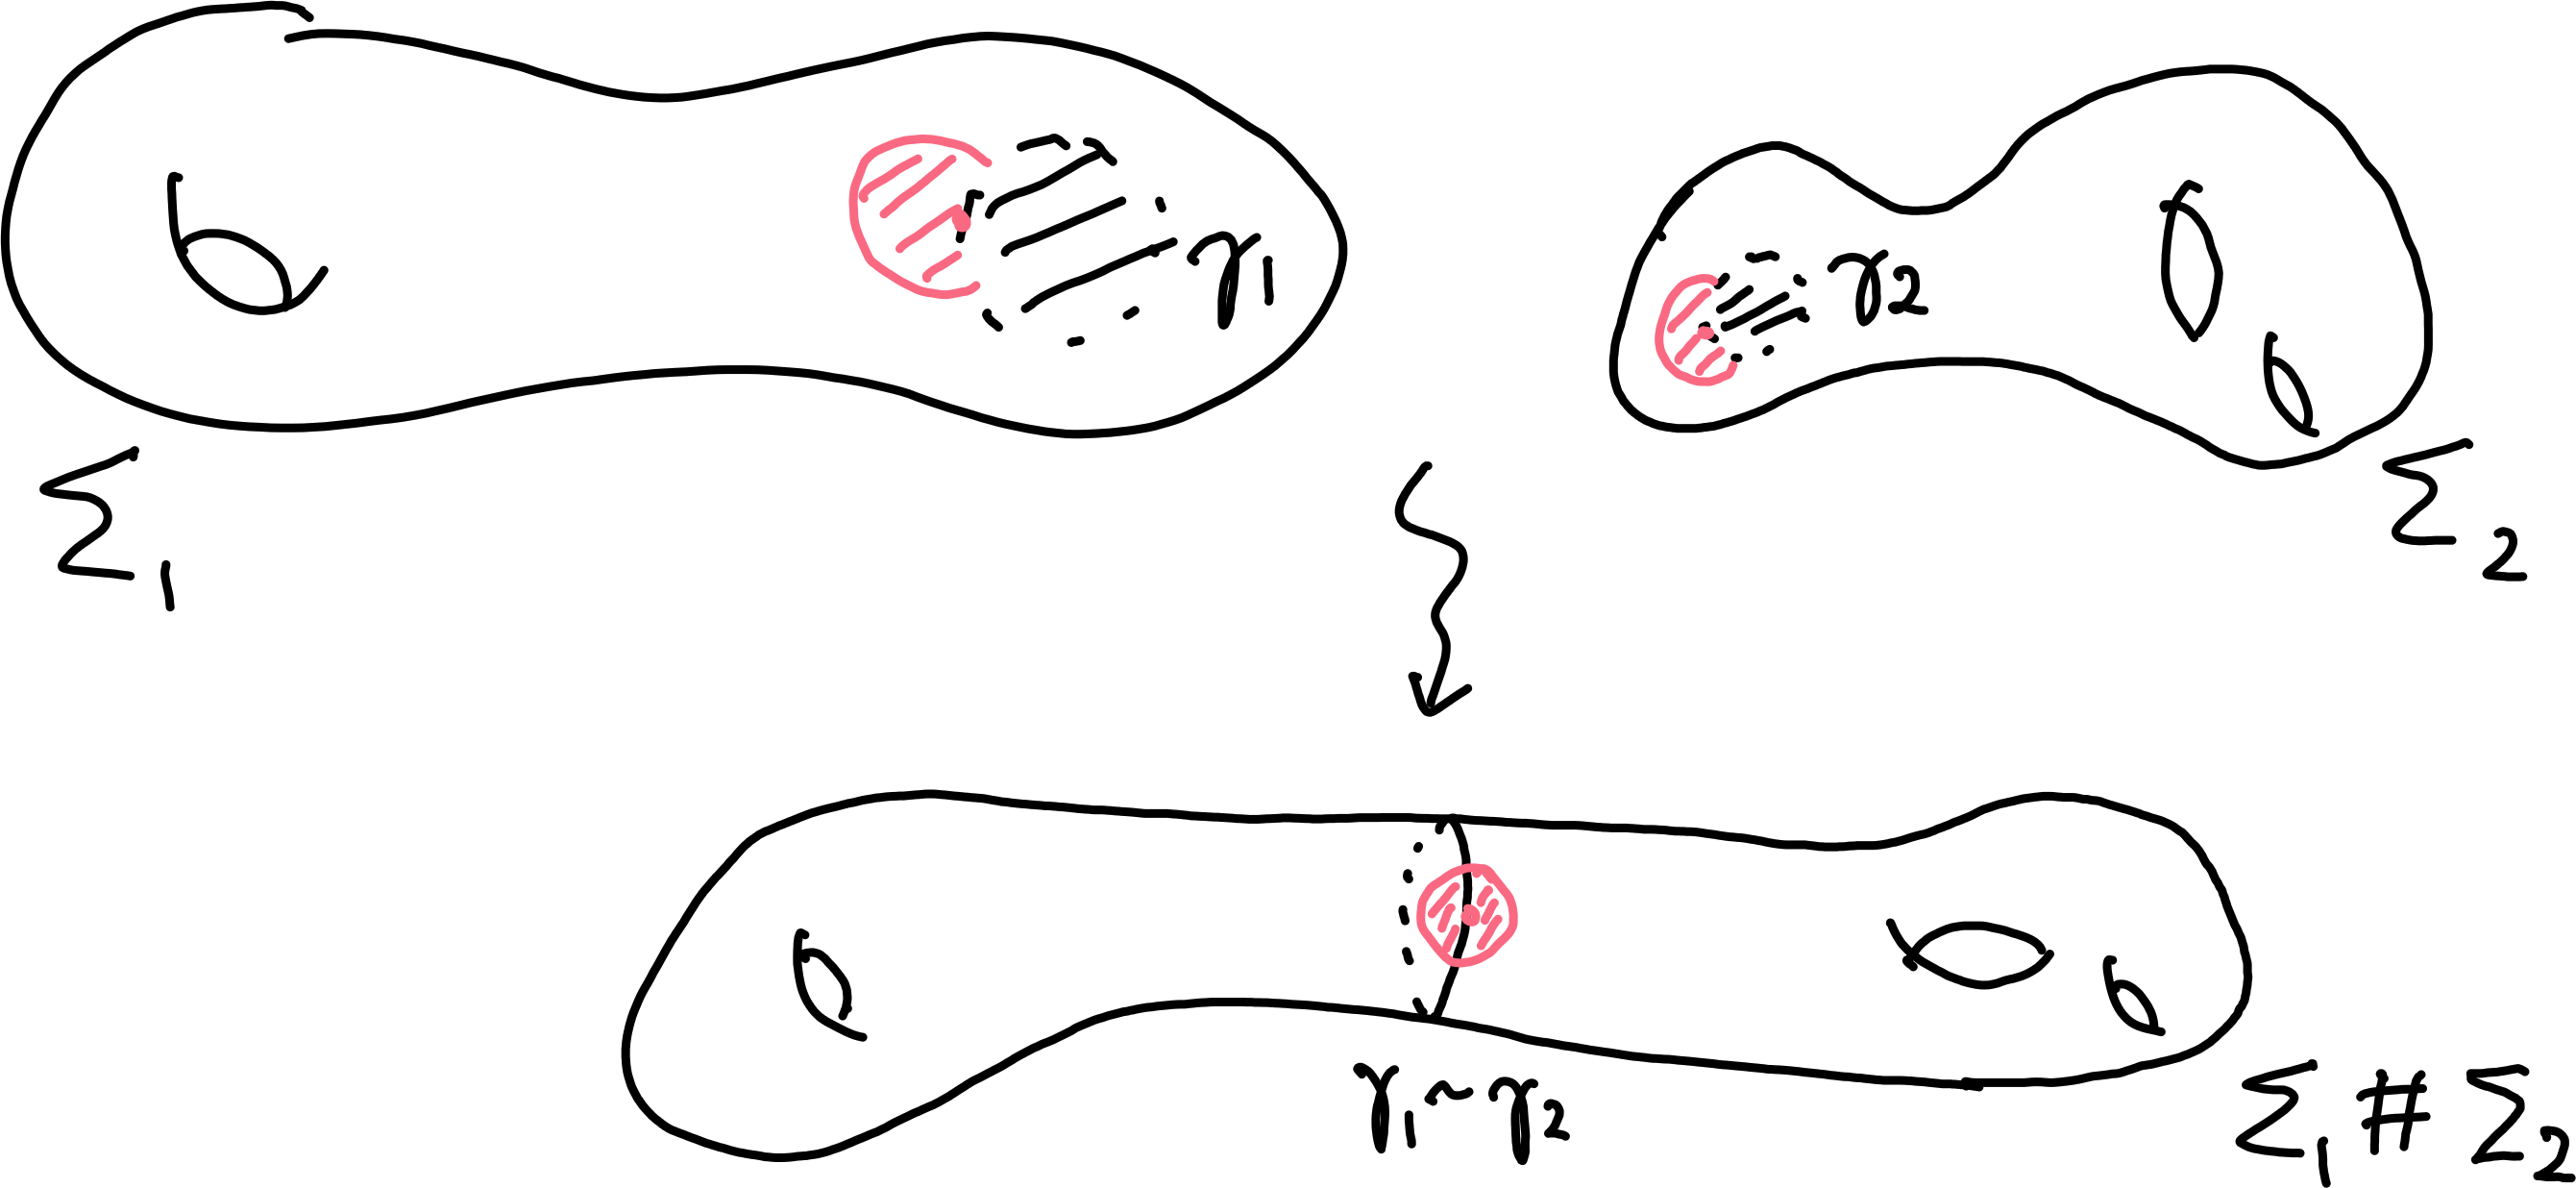
\includegraphics[height=5cm]{01-connectedsum} 
		\par
	}
	Explicitly, take $\Sigma_1 \setminus D_1 \indep\footnote{Disjoint Union} \Sigma_2 \setminus D_2$ and impose a quotient relation by identifying $\theta \in \partial D_1 \sim \theta \in \partial D_2$ where $\theta$ is an angle parametrising $S^1 = \partial D_i$, $\partial D_i$ is the boundary of $D_i$.
	The result $\Sigma_1 \connect \Sigma_2$ is called the \vocab{connected sum} of $\Sigma_1, \Sigma_2$.

	In principle this depends on many choices and takes some effort to prove that it is well-defined.

	% Typically, the information about where the discs were removed from is discarded when considering the connect sum.
	% The connect sum of two topological surfaces is a topological surface.
\end{example}

\begin{lemma}
	The connected sum $\Sigma_1 \connect \Sigma_2$ is a topological surface.
\end{lemma} 

\begin{proof}
	Not proved in this course, if you want to learn more try `Introduction to topological manifolds' by Jack Lee.
\end{proof} 

\begin{example}
	Consider the following octagon.
	\tikzfig{double_torus_polygon}
	The associated quotient space $\faktor{P}{\sim}$ can be seen to be homeomorphic to a surface with two holes, known as a double torus.
	All vertices are identified as the same vertex in the quotient space.
	We can cut the octagon along a diagonal, leaving two topological surfaces which are homeomorphic to a torus.
	\begin{center}
		\tikzfig{double_torus_polygon_expanded} $\mapsto$ \tikzfig{torus_polygon_with_loop}
	\end{center}
	Thus, the connected sum of the two half-octagons are the connected sum of two toruses.
\end{example}

\begin{example}
	Consider the following square.
	\tikzfig{rp2_polygon}
	This is homeomorphic to the real projective plane $\mathbb R \mathbb P^2$.
	This is because we identify points on the boundary with their antipodes, when interpreting the square as the closed disc $B(0,1)$.
	The real projective plane was constructed by identifying points on the unit sphere with their antipodes.
	Thus, we can construct a homeomorphism by considering only points in the upper hemisphere (taking antipodes as required), and then orthographically projecting onto the $xy$ plane.
	Under this transformation, points on the boundary are identified with their antipodes as required.
\end{example}

\subsection{Subdivisions}

\begin{definition}[Subdivision]
	A \vocab{subdivision} of a compact topological surface $\Sigma$ comprises
	\begin{enumerate}
		\item a finite subset $V \subseteq \Sigma$ of vertices;
		\item a finite subset of edges $E = \qty{e_i : [0,1] \to \Sigma}$ s.t. 1) each $e_i$ is a continuous injection on its interior and $e_i\inv V = \{0, 1\}$, the endpoints.
		2) $e_i, e_j$ have disjoint images except perhaps at their endpoints.
		\item we require that each connected component of $\Sigma \setminus \qty(\cup_i e_i [0, 1] \cup V)$ is homeomorphic to an open disc called a \vocab{face}.
		      In particular, the closure of a face has boundary $\overline F \setminus F$ lying in $\qty(\cup_i e_i [0, 1] \cup V)$.
	\end{enumerate}
\end{definition}

\begin{definition}[Triangulation]
	We say that a subdivision is a \vocab{triangulation} if each closed face (closure of a face) contains exactly three edges, and two closed faces are disjoint, meet at exactly one edge or just one vertex.
\end{definition} 

\begin{example}
	A cube displays a subdivision of $S^2$.
	A tetrahedron displays a triangulation of $S^2$.
\end{example}

\begin{example}
	We can display subdivisions of surfaces constructed from polygons.
	\tikzfig{torus_polygon}
	This is a subdivision of a torus with one vertex, two edges, and one face.
	We can construct additional subdivisions of a torus, for example:
	\begin{center}
		\tikzfig{torus_polygon_subdivided} \quad \tikzfig{torus_polygon_triangulated}
	\end{center}
	The first of these examples is not a triangulation, since the two faces meet in more than one edge.
	The second is a triangulation.
\end{example}

\begin{remark}
	The following is a very degenerate subdivision of $S_2$.
	\tikzfig{s2_degenerate}\footnote{This is not a circle, its a 2-sphere.}
	This has one vertex, no edges, and one face.
\end{remark}

\subsection{Euler classification}
\begin{definition}[Euler Characteristic]
	The \vocab{Euler characteristic} of a subdivision is
	\begin{align*}
		\#\footnote{The number/size of the set} V - \# E + \# F
	\end{align*}
\end{definition}

\begin{theorem}
	\begin{enumerate}
		\item Every compact topological surface has a subdivision (and indeed triangulations).
		\item The Euler characteristic is invariant under choice of subdivision, and is topologically invariant of the surface (depends only on the homeomorphism type of $\Sigma$).
	\end{enumerate}
	Hence, we might say that a surface has a particular Euler characteristic, without referring to subdivisions.
	We write this $\chi(\Sigma)$.
\end{theorem}

\begin{remark}
	It is not trivial to prove part (i).
	For part (ii), note that subdivisions can be converted into triangulations by constructing triangle fans.
	\tikzfig{triangle_fan}
	Triangulations can be related by local moves, such as
	\tikzfig{triangulation_local_move}
	It is easy to check that both of these moves do not change the Euler characteristic.
	However, it is hard to make this argument rigorous, and it does not give much explanation for why the result is true.
	In Part II Algebraic Topology, a more advanced definition of the Euler characteristic is given, which admits a more elegant proof.
\end{remark}

\begin{proof}
	No proof will be given.
\end{proof} 

\begin{example}
	The Euler characteristic of $S^2$ is $\chi(S^2) = 2$.
\end{example}

\begin{example}
	For the torus, $\chi(T^2) = 0$.
\end{example} 

\begin{example}
	If $\Sigma_1, \Sigma_2$ are compact surfaces, then the connected sum $\Sigma_1 \connect \Sigma_2$ can be constructed by removing a face of a triangulation, then gluing together the boundary circles (three edges) in a way that matches the edges.

	Then the connected sum inherits a subdivision, and we can find that it has Euler characteristic $\chi(\Sigma_1 \connect \Sigma_2) = \chi(\Sigma_1) + \chi(\Sigma_2) - 2$, where the remaining term corresponds to the two faces that were removed; the changes of three vertices and three edges cancel each other.

	In particular, a surface $\Sigma_g$ with $g$ holes can be written $\bigconnect_{i=1}^g T^2$, so $\chi(\Sigma_g) = 2 - 2g$.
	We call $g$ the \vocab{genus} of $\Sigma$.
\end{example} 